\chapter{Lo \textit{stage}}
\label{cap:lo-stage}



\section{Il ruolo degli stage nell'azienda}
Zero12 crede fortemente nella collaborazione tramite \textit{stage} con gli studenti dell'Università di Padova. Grazie all'evento \gls{stageItg}, un' evento promosso da Confindustria Veneto Est e l'Universita degli studi di Padova, l'azienda permette agli studenti di svolgere progetti di \textit{stage} presso la loro sede.
Gli stage per loro, rappresentano una doppia opportunità. Da una parte l’azienda ha modo di inserire nuove figure professionali nel proprio organico, dall’altra gli studenti che hanno la possibilità di inserirsi nel mondo del lavoro e poter applicare le proprie conoscenze acquisite durante il percorso di studi.
Durante le otto settimane di \textit{stage} ho avuto l’occasione di conoscere quasi tutti i membri dell’azienda, comprendere il loro metodo di lavoro e mettere in pratica le mie conoscenze. Il mio percorso è stato guidato dal \textit{tutor} aziendale, che mi è stato assegnato, coordinando le varie attività da svolgere e fornendo supporto in caso di dubbi o problemi. 
L'accoglienza e l'ambiente di lavoro sono molto positivi, dimostrando una grande attenzione nei confronti degli stagisti. 
Questa attenzione è testimoniata anche dalla presenza di molti dipendenti che attualmente lavorano in azienda dopo aver svolto uno \textit{stage} in Zero12.
I progetti assegnati durante gli \textit{stage} vengono concepiti in base a delle reali esigenze interne all’azienda. Essi sono mirati a migliorare la comunicazione tra i collaboratori, automatizzare delle attività manuali e a migliorare la qualità del lavoro svolto.

\section{Introduzione al progetto}
Durante il mio \textit{stage} ho avuto modo di lavorare non solo al progetto inizialmente proposto inzialmente, ma anche allo sviluppo di progetto aggiuntivo, streattamene correlato al primo.
Di seguito descrivo il progetto inizialmente proposto dall'azienda all'evento \gls{stageItg} e il progetto aggiuntivo concepito e sviluppato durante lo \textit{stage}.
\subsection{Sistema di proposte di risoluzioni a \textit{ticket} Jira}
L'idea del mio progetto nasce come strumento che l'azienda può utilizzare per velocizzare alcuni processi, che però può essere estesa ai clienti dell'azienda stessa. Nel contesto del progetto, viene immaginata un'azienda che vende componenti \textit{hardware}. 
Nel caso di problematiche con la componente comprata, il cliente chiama il servizio clienti dell'azienda, e l'operatore inserisce un \textit{ticket} all'interno dell'\gls{itsg} aziendale. Immaginando questa iterazione tra cliente e addetto al servizio clienti, i \textit{ticket} inseriti all'interno del sistema saranno numerosi e molto simili tra loro. 
Questo proietta al fatto che a nuovi \textit{ticket} inseriti, molto probabilmente ci saranno dei \textit{ticket} simili già risolti in passato. 
Ed è qui che da Zero12 nasce l'idea di creare un sistema di proposte di risoluzioni automatiche di \textit{ticket} inseriti all'interno di un \gls{itsg}, che permetta di velocizzare il processo di risoluzione del problema. Le proposte di risoluzione vengono generate grazie all'utilizzo della IA Generativa, in base al contesto dei \textit{ticket} precedentemi inseriti.

\begin{figure}[H]
    \centering
    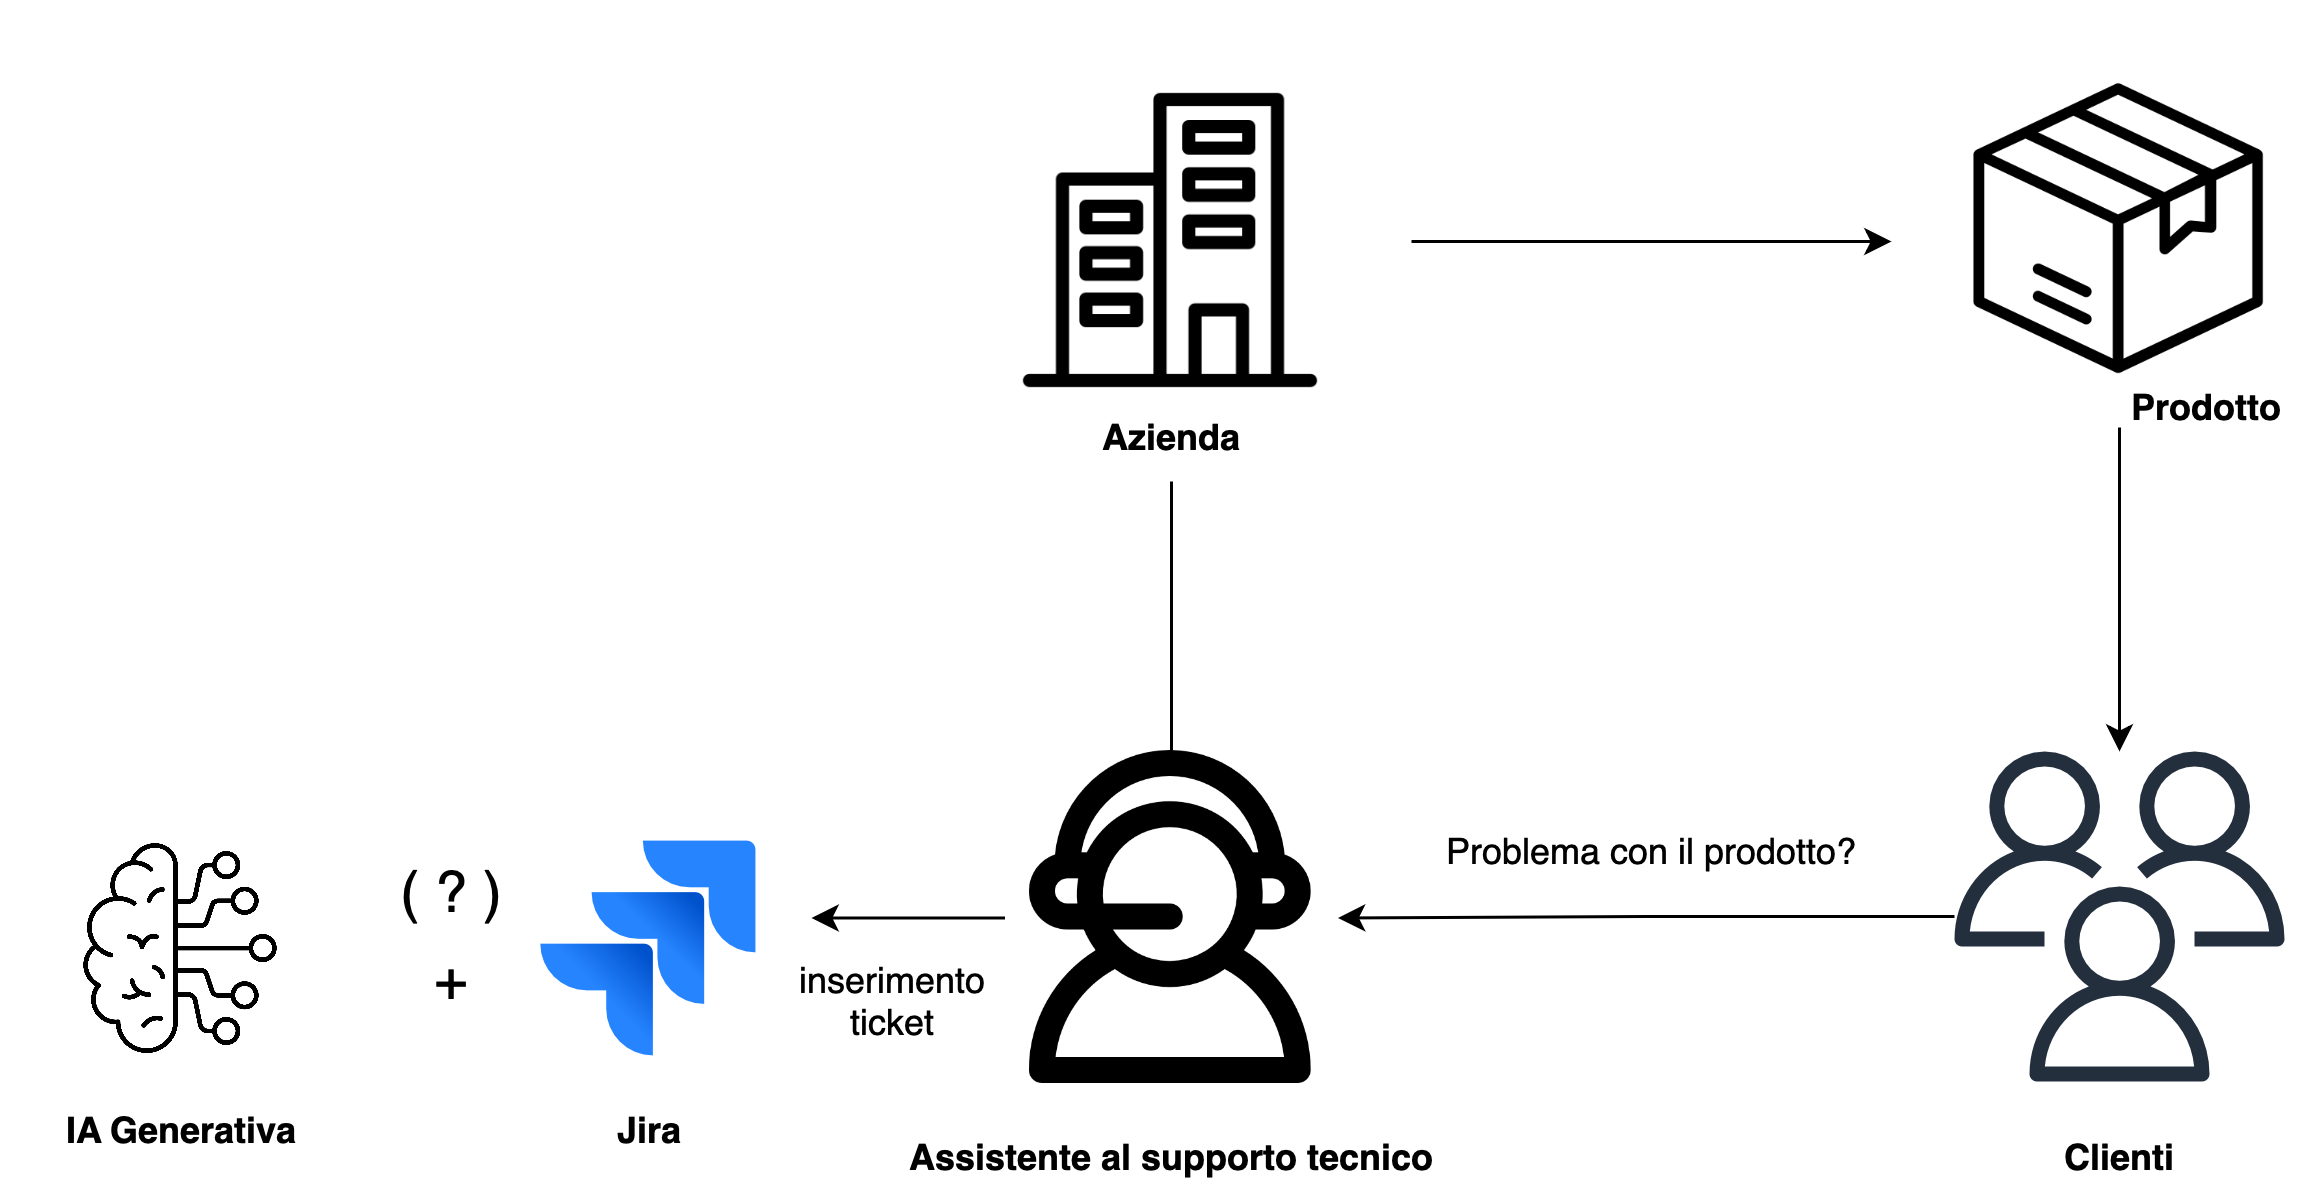
\includegraphics[width=0.8\textwidth]{ideaJira.png}
    \caption{Schema che rappresenta l'idea del progetto}
    \label{fig:ideaJira}
\end{figure}
\subsection{\textit{Chatbot} per proposte di risoluzioni}
Durante lo sviluppo del progetto descritto nel paragrafo precedente, è nata l'idea di creare un ulteriore strumento che permetta di svolgere la stessa funzionalità del sistema di proposte di risoluzioni, ma in modo differente. Lo strumento aggiuntivo è un \textit{chatbot} che permette di generare proposte di risoluzione, in base al testo di un \textit{ticket} inserito all'interno della chat. 
Sempre grazie alla IA Generativa, il \textit{chatbot} genera proposte di risoluzione in base al contesto dei \textit{ticket} precedentemente inseriti. A differenza del sistema Jira, il \textit{chatbot} propone le risoluzioni in modo più descrittivo e dettagliato, e permette di interagire con l'assistente virtuale, per ottenere informazioni più dettagliate.
\section{Importanza del progetto}
Descrizione di come il progetto proposto dall'azienda sia importante per l'azienda stessa

\section{Vincoli dello \textit{stage}}
\subsection{Vincoli di rendicontazione}
Descrizione dei documenti scritti e della presentazione effettuate
\subsection{Vincoli temporali}
Analisi delle tempistiche e delle scadenze da rispettare durante lo stage.


\section{Scelta dello \textit{stage}}
Spiegazione delle ragioni per cui ho scelto questo stage tra le varie offerte.
Verranno elencati anche gli obiettivi personali.
